\documentclass[journal]{IEEEtran}
\usepackage[a5paper, margin=10mm]{geometry}
%\usepackage{lmodern} % Ensure lmodern is loaded for pdflatex
\usepackage{tfrupee} % Include tfrupee package


\setlength{\headheight}{1cm} % Set the height of the header box
\setlength{\headsep}{0mm}     % Set the distance between the header box and the top of the text


%\usepackage[a5paper, top=10mm, bottom=10mm, left=10mm, right=10mm]{geometry}

%
\setlength{\intextsep}{10pt} % Space between text and floats

\makeindex


\usepackage{cite}
\usepackage{amsmath,amssymb,amsfonts,amsthm}
\usepackage{algorithmic}
\usepackage{graphicx}
\usepackage{textcomp}
\usepackage{xcolor}
\usepackage{txfonts}
\usepackage{listings}
\usepackage{enumitem}
\usepackage{mathtools}
\usepackage{gensymb}
\usepackage{comment}
\usepackage[breaklinks=true]{hyperref}
\usepackage{tkz-euclide} 
\usepackage{listings}
\usepackage{multicol}
\usepackage{xparse}
\usepackage{gvv}
%\def\inputGnumericTable{}                                 
\usepackage[latin1]{inputenc}                                
\usepackage{color}                                            
\usepackage{array}                                            
\usepackage{longtable}                                       
\usepackage{calc}                                             
\usepackage{multirow}                                         
\usepackage{hhline}                                           
\usepackage{ifthen}                                               
\usepackage{lscape}
\usepackage{tabularx}
\usepackage{array}
\usepackage{float}
\usepackage{ar}
\usepackage[version=4]{mhchem}


\newtheorem{theorem}{Theorem}[section]
\newtheorem{problem}{Problem}
\newtheorem{proposition}{Proposition}[section]
\newtheorem{lemma}{Lemma}[section]
\newtheorem{corollary}[theorem]{Corollary}
\newtheorem{example}{Example}[section]
\newtheorem{definition}[problem]{Definition}
\newcommand{\BEQA}{\begin{eqnarray}}
\newcommand{\EEQA}{\end{eqnarray}}

\theoremstyle{remark}


\begin{document}
\bibliographystyle{IEEEtran}
\onecolumn

\title{5.8.25}
\author{INDHIRESH S- EE25BTECH11027}
\maketitle


\renewcommand{\thefigure}{\theenumi}
\renewcommand{\thetable}{\theenumi}

\textbf{Question}.One says, "Give me a hundred, Friend! I shall then become twice as rich as you ". The other "if you give me ten, i shall be six times as rich as you ". Tell me What is the amount of their (respective) capital? [From the bijaganita of Bhaskara II].\\
\textbf{Solution}:\\
Let us solve the given equation theoretically and then verify the solution computationally. \\
Let an amount with Friend 1 be $a$ and amount with Friend 2 be $b$\\
From given information:
\begin{align}
   a+100=2(b-100)
\end{align}
\begin{align}
 a-2b=-300
\end{align}
And
\begin{align}
  b+10=6(a-10)
 \end{align}

\begin{align}
   b+10=6a-60;
\end{align}

\begin{align}
    6a-b=70
\end{align}
By combining the Eq.2 and Eq.5 we get
\begin{align}
  \myvec{1&-2\\6&-1}\Vec{x}=\myvec{-300\\70}
\end{align}
Where
\begin{align}
\Vec{x}=\myvec{a\\b}
\end{align}
\begin{align}
     \augvec{2}{1}{1 & -2 & -300\\6 & -1 & 70} \xleftrightarrow{R_2\longleftarrow R_2-6R_1} \augvec{2}{1}{1 & -2 & -300\\0 & 11 & 1870}
\end{align}
\begin{align}
    \augvec{2}{1}{1 & -2 & -300\\0 & 11 & 1870} \xleftrightarrow{R_2\longleftarrow \frac{1}{11}R_2} \augvec{2}{1}{1 & -2 & -300\\0 & 1 & 170}
\end{align}
\begin{align}
   \augvec{2}{1}{1 & -2 & -300\\0 & 1 & 170} \xleftrightarrow{R_1\longleftarrow R_1+2R_2} \augvec{2}{1}{1 & 0 & 40\\0 & 1 & 170}
\end{align}
\begin{align}
    \Vec{x}=\myvec{40\\170}
\end{align}

\begin{align}
a=40\;\;and\;\;b=170
  \end{align}
The amount with Friend 1 = 40 \\
The amount with Friend 2 = 170



From the figure it is clearly verified that the theoretical solution matches with the computational solution.\\
\begin{figure}[h]
    \centering
    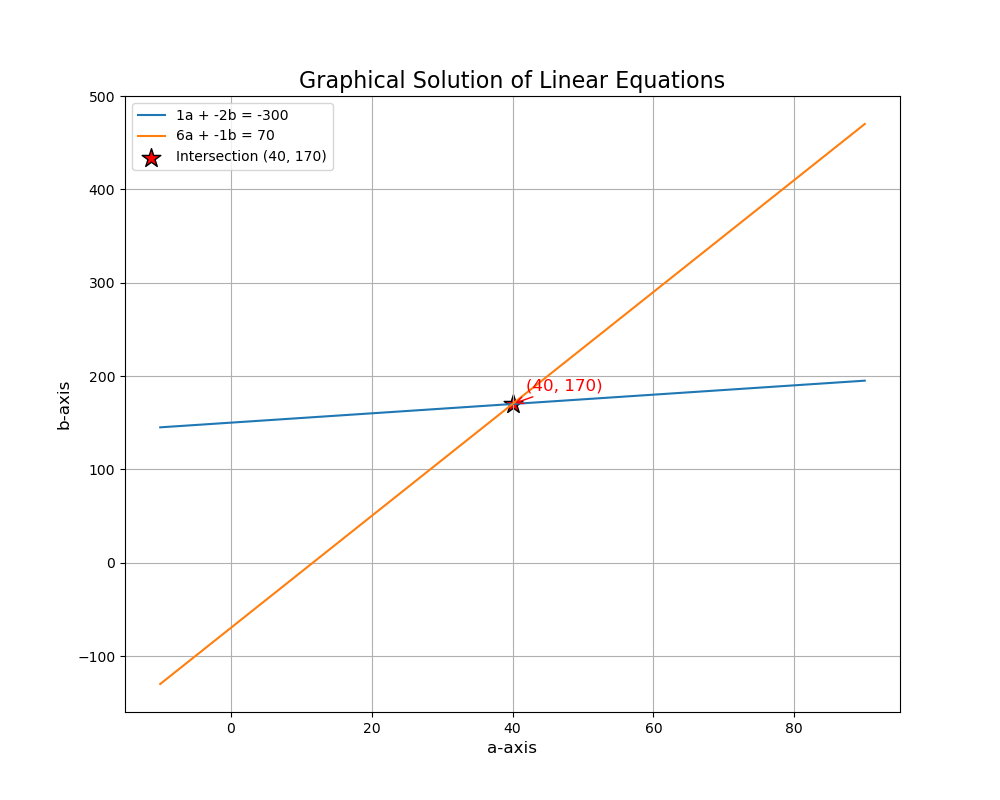
\includegraphics[height=0.5\textheight, keepaspectratio]{figs/figure1.png}
    \label{figure_1}
\end{figure}

\end{document}